% !TeX encoding = UTF-8
% !TeX TS-program = xelatex
% !TeX engine=xelatex
% !TeX spellcheck = en_GB
% !TeX root = ../Herbstrith-H10_over_AI.tex

In this section I closely follow the lecture notes on the subject by
\textcite{Mueller2016}.

\begin{defin}
  A \emph{(decision) problem} is a subset of the set of finite
  $\zer$-$\one$-strings $\lbrace \zer, \one \rbrace^*$ including the
  empty string $λ$. One calls $\lbrace \zer, \one \rbrace$
  \emph{alphabet} and its elements \emph{bits.}
\end{defin}

One immediate objection against this definition is that not all problems
arise as subsets of these strings. However, such problems $Q$ are
captured up to an encoding.

\[ \enc{\cdot} : Q → \lbrace \zer, \one \rbrace^*\]

One usually does not concern oneself with the details of this encoding.
However, the encoding should capture the structure of the problem---a notion
that will be made precise in \cref{sec:computable structures}.

\begin{exam}
  Consider the problem of deciding whether a finite simple graph is
  connected or not. If one demands the vertex set to be of the form
  $\set{0, 1, …, n}$, then the set of all graphs can be encoded
  as the set of the respective adjacency matrices written as a string
  \[
    b_{00}b_{01} …b_{0n}b_{10}…b_{nn}
  \]
  of length $(n + 1)^2$, where $b_{ij} = \one$ if and only if the
  vertices $i$ and $j$ are connected.
\end{exam}

\begin{defin}
  A \emph{Turing machine} $\mathbb A$ on the \emph{alphabet}
  $A = \lbrace \sta, \emp, \zer, \one \rbrace$ is a tuple $(S, δ)$,
  where $\sstart, \shalt ∈ S$ is a finite non-empty set, called
  \emph{set of states}, and
  \[
    δ: S × A → S × A × \lbrace -1, 0, 1 \rbrace
  \]
  is called \emph{transition function}. If $δ(s, a) = (s', b, m)$, one
  demands that the following axioms are satisfied

  \begin{thmlist}
  \item
    $a = \sta$ if and only if $b = \sta$,
  \item
    If $a = \sta$, then $m ≠ -1$, and
  \item
    If $s = \shalt$, then $s' = \shalt$, $a = b$ and $m = 0$.
  \end{thmlist}
\end{defin}

Informally, one can think of a Turing machine as a device, consisting of a
\emph{work-tape} and a \emph{head}. The work-tape stores all the information in
cells arranged in a consecutive order. Each of these cells contains a letter
from the alphabet.

Let us look at the example of the Turing machine in \cref{fig:Turing machine}.
During the run of the machine the head reads the symbol $\zer$ at the current
position and the machine evaluates the transition function $δ$ at $\zer$ and the
current state $\state{overflow}$. Now assume that
\[
  δ(\state{overflow}, \zer) = (\state{return}, \one, -1).
\]
One interprets this in the following way. The Turing machine changes its state
to $\state{return}$, the head writes $\one$ in the current cell and moves one
cell to the left. The movement is determined by the last item of the triple
$δ(\state{overflow}, \zer)$, where $-1$ indicates moving to the left, $1$
indicates moving to the right, and $0$ indicates not moving at all.

\begin{figure}
  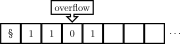
\includegraphics{res/turing_add1_4}
  \caption{A Turing machine}
  \label{fig:Turing machine}
\end{figure}

\begin{defin}
  Let $\mathbb A = (S, δ)$ be a Turing machine. A \emph{configuration}
  of $\mathbb A$ is a triple $(s, j, c) ∈ S × ℕ × A^ℕ$. It reflects
  the current state of $\mathbb A$, the current position of its
  head, and the content of its work-tape.
\end{defin}

A configuration of the form $(\shalt, 0, c)$ is called \emph{halting}. A
\emph{start configuration} is of the form $(\sstart, 0, c)$ such that $c(0) =
\sta$ and there exists an $n ∈ ℕ$ such that $c(i) = \emp$ if and only if $i >
n$. This means that in a start configuration the work-tape reads
\[
  \sta x_1 x_2 … x_n \emp \emp …
\]
It will be very convenient to identify the finite string $x_1…x_n$ with this
tape content.

\begin{defin}
  One writes $(s, j, c) \vdash_1 (s', j', c')$ and calls $(s', j', c')$ a
  \emph{successor configuration} of $(s, j, c)$ if there exists an $m ∈ \lbrace
  -1, 0, 1 \rbrace$ such that

  \begin{itemize}
  \item
    $δ(s, c) = (s', c', m)$,
  \item
    $j' = j + m$, and
  \item
    $c'(ℓ) = c(ℓ)$ for all $ℓ ≠ j$.
  \end{itemize}

  This relation makes the set of all configurations of $\mathbb A$ into a
  directed graph. A \emph{run} of $\mathbb A$ on $x$ is a path in this directed
  graph starting at the start configuration $(\sstart, 0, x)$. A run of
  $\mathbb A$ on $x$ is \emph{halting} or \emph{complete} if it reaches a
  halting configuration $(\shalt, 0, y)$. In this case I write $\mathbb A (x) =
  y$.
\end{defin}

I will denote Turing machines using listings, where the fact that
$δ_\text{delta} (\state{state}, b) = (\state{state'}, c, m)$ is encoded by

\begin{lstlisting}
delta "state" c = ("state'", c', m)
\end{lstlisting}

Variables \verb+c+ match all possible states or characters in the alphabet
respectively. However, I follow the convention that if an assignment of
variables matches more than one pattern, the first matching pattern is chosen.
This means that
%
\begin{lstlisting}
delta "state" 1 = ("state'", 1, 1)
delta "state" c = ("state''", c, 0)
\end{lstlisting}
%
should be interpreted as
%
\[ δ(s, c) =
  \begin{cases}
    (\state{state'}, \one, 1) & \text{if } s=\state{state} ∧ c = \one\\
    (\state{state''}, c, 0) & \text{if } s=\state{state} ∧ c ≠ \one
  \end{cases}.
\]

See \cref{app:turing} on how to simulate Turing machines
using the \emph{Haskell} programming language.

\begin{exam}
    Consider the Turing machine $\mathbb A_\text{add1} = (\lbrace \sstart,
    \shalt, \state{overflow}, \state{return}, \state{error} \rbrace,
    δ_\text{add1})$ that adds $1$ to a (possibly zero-patched) binary
    representation of a natural number $n$. Its transition function is described
    in \cref{lst:add1}. The last line of the program ensures, that $δ$ is a
    total function, as it matches all remaining pairs of states and
    characters and lets the machine enter the state $\state{error}$. The
    complete run of $\mathbb A_\text{add1}$ on $\one\one\zer\one$ can be seen in
    \cref{fig:complete run}.
\end{exam}

\lstinputlisting[float, frame=tb,
                 caption=A Turing machine adding one to the input string,
                 label=lst:add1]{./listings/add1.hs}

\begin{figure*}
    \begin{subfigure}{.5\textwidth}
        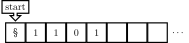
\includegraphics{res/turing_add1_1}
        \caption{$δ(\sstart, \sta) = (s_\text{overflow}, \sta, 1)$}
    \end{subfigure}

    \begin{subfigure}{.5\textwidth}
        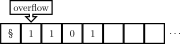
\includegraphics{res/turing_add1_2}
        \caption{$δ(s_\text{overflow}, \one) = (s_\text{overflow}, \one, 1)$}
    \end{subfigure}

    \begin{subfigure}{.5\textwidth}
        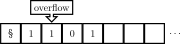
\includegraphics{res/turing_add1_3}
        \caption{$δ(s_\text{overflow}, \one) = (s_\text{overflow}, \one, 1)$}
    \end{subfigure}

    \begin{subfigure}{.5\textwidth}
        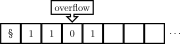
\includegraphics{res/turing_add1_4}
        \caption{$δ(s_\text{overflow}, \zer) = (s_\text{return}, \one, -1)$}
    \end{subfigure}

    \begin{subfigure}{.5\textwidth}
        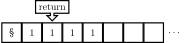
\includegraphics{res/turing_add1_5}
        \caption{$δ(s_\text{return}, \one) = (s_\text{return}, \one, -1)$}
    \end{subfigure}

    \begin{subfigure}{.5\textwidth}
        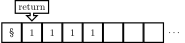
\includegraphics{res/turing_add1_6}
        \caption{$δ(s_\text{return}, \one) = (s_\text{return}, \one, -1)$}
    \end{subfigure}

    \begin{subfigure}{.5\textwidth}
        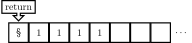
\includegraphics{res/turing_add1_7}
        \caption{$δ(s_\text{return}, \sta) = (s_\text{halt}, \sta, 0)$}
    \end{subfigure}

    \begin{subfigure}{.5\textwidth}
        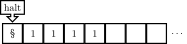
\includegraphics{res/turing_add1_8}
        \caption{$δ(s_\text{halt}, \sta) = (s_\text{halt}, \sta, 0)$}
    \end{subfigure}

    \caption{The complete run of $\mathbb A_\text{add1}$ on $\one\one\zer\one$}
    \label{fig:complete run}
\end{figure*}

\begin{defin}
    Let $\mathbb A$ be a Turing machine.

    \begin{thmlist}
        \item
          $\mathbb A$ \emph{computes} the partial function that maps each
          $x$ with a complete run to $\mathbb A(x)$ and is undefined for all
          other strings.
        \item
          $\mathbb A$ \emph{accepts} all $x$ such that
          $\mathbb A(x) = \one$ and \emph{rejects} them if
          $\mathbb A(x) = \zer$.
        \item
          A partial function on $\lbrace \zer, \one \rbrace^*$ is
          \emph{computable} if there is a Turing machine computing it. Sometimes
          computable functions are referred to as \emph{recursive} or
          \emph{efficient} functions.
        \item
          A subset of $\lbrace \zer, \one \rbrace^*$, i.e. a
          problem, is \emph{decidable} if there is a Turing machine computing
          its characteristic function.
        \item
          A problem is called \emph{semi-decidable} or \emph{computably
          enumerable} if there is a Turing machine accepting precisely the
          elements of the problem.
    \end{thmlist}
\end{defin}

The last item of the definition above means that a problem is
semi-decidable if there is a Turing machine affirming membership of the
corresponding set but it might not be able to refute membership.

Note that every finite problem is decidable by a Turing machine that reads the
tape content and checks at every step whether there are elements in the problem
that start with the tape content the machine has read. After $n + 1$ steps,
where $n$ denotes the length of the longest string in the problem, the machine
stops at the latest.

\begin{lem} \label{lem:composition of Turing machines}
  Let $\mathbb A_1 = (S_1, δ_1)$ and $\mathbb A_2 = (S_2, δ_2)$ be Turing
  machines computing $f_1: D_1 → \set{\zer, \one}^*$ and $f_2: D_2 → \set{\zer,
  \one}^*$ respectively ($D_1, D_2 \subseteq \set{\zer, \one}^*$). Then there
  exists a Turing machine $\mathbb A_{f_2 \circ f_1}$ computing the partial
  function $f_2 \circ f_1: D_1 ∩ f_1^{-1}(D_2) → \set{\zer, \one}^*$ obtained by
  composing $f_1$ and $f_2$.
\end{lem}
\begin{proof}
  One constructs $\mathbb A_{f_2 \circ f_1}$ from $\mathbb A_1$ and $\mathbb
  A_2$ as follows. Let $S_1 = \set{\sstart, \shalt} \sqcup S_1'$ and $S_2 =
  \set{\sstart, \shalt} \sqcup S_2'$, then set $S = \set{\sstart, \shalt} \sqcup
  S_1' \sqcup S_2' \sqcup \set{\state{compose}}$, where $\sqcup$ denotes the
  disjoint union. Now set for $c ∈ A$
  %
  \begin{align*}
    δ (s, c) &=
      \begin{cases}
        δ_1 (s, c) & \text{if } s ∈ S_1' ∪ \set\sstart \\
        (\state{compose}, c', m) & \text{if } s ∈ S_1 \text{ and } δ_1(s, c) = (\shalt, c', m)\\
        δ_2 (s, c) & \text{if } s ∈ S_2' ∪ \set\shalt \\
      \end{cases}, \\
    δ (\state{compose}, c) &= δ_2 (\sstart, c).
  \end{align*}
  %
  Then $\mathbb A_{f_2 \circ f_1} = (S, δ)$ computes $f_1 \circ f_2$ because $δ$
  is defined to first run the program of $\mathbb A_1$ and if this machine would
  reach a halting state run $\mathbb A_2$.
\end{proof}
% IDEA
\todo{Maybe: A semi-decidable set is decidable iff its complement is semi-decidable}

\begin{exam}
    One can encode a natural number $n$

    \begin{exlist}
    \item \label{ex:tally encoding}
      in tally notation
      \begin{align*}
        n & ↦ \underbrace{\one…\one}_{n\text{-times}}, \quad \text{if } n > 0 \\
        0 & ↦ λ
      \end{align*}
    \item
      by its binary representation
      \begin{align*}
          n = 2^k + \sum_{i = 0}^{k-1} b_i 2^i & ↦ b_0…b_{k-1}\one, \quad
              \text{if } n > 0\\
                                             0 & ↦ \zer,
      \end{align*}
      or
    \item \label{ex:omega encoding}
      by a shifted and truncated form of its binary representation
      \begin{align*}
        n = 1 + \sum_{i = 0}^k b_i 2^i & ↦ b_0…b_k, \quad \text{if } n > 0\\
                                     0 & ↦ λ
      \end{align*}

      In other words, $n$ is mapped to the $n$-th string if one orders $\lbrace
      \zer, \one \rbrace ^ ℕ$ lexicographically. Following a tradition in
      logics I denote $ℕ$ under this last encoding by $ω$.
    \end{exlist}

    In either case the set obtained by encoding $ℕ$ is easily seen to be
    decidable. In the first case, check that the string contains only copies
    of the bit $\one$. Indeed, this can be achieved by the Turing machine
    %
    \[\mathbb A_\text{tally} =
      ( \lbrace \sstart, \shalt, \scheck, \state{accept}, \state{reject},
        \state{rejectMR}, \state{error} \rbrace, δ),\]
    %
    whose transition function is displayed in \cref{lst:tally encoding}.

    In the second case it suffices to check that the string has length $1$
    or ends in an $\one$, and in the third case every string is accepted.
\end{exam}

\lstinputlisting[float, frame=tb,
                 caption=A Turing machine checking whether the input is tally-encoded,
                 label=lst:tally encoding]{./listings/tally.hs}

Taking another look at the definition of computability, one sees that only unary
functions defined on subsets of $ω$, mapping to subsets of $ω$ can be
computable. However, one can easily extend this to functions on multiple
variables, by encoding tuples in $ω \times ω$ by elements of $ω$ in such a way,
that the projections $p_i: \enc{(x_1, x_2)} ↦ x_i$  for $i ∈ \lbrace 0, 1
\rbrace$ are uniformly computable. This means, there are injective pairing
functions $ω^2 → ω$ and Turing machines $\mathbb P_1, \mathbb P_2$
computing $p_1$ or $p_2$ respectively. Clearly if one has a pairing function $ℕ^2 → ℕ$ then one immediately obtains a pairing function $ω^2 → ω$
by composing with the encoding function.

\begin{exam}[Pairing functions]
  \begin{exlist}
    \item\label{ex:tally pairing}
    Using tally notation on can encode $(n, m) ∈ ℕ^2$ by
    \[
      ⟨\enc{n}, \enc{m}⟩ = \underbrace{\one … \one}_{n\text{-times}} \zer \underbrace{\one … \one}_{m\text{-times}}
    \]

    \item A simple pairing function encodes the pair $(b_1b_2…b_n, c_1c_2…c_m) ∈ ω^2$

    \[ ⟨b_1b_2…b_n, c_1c_2…c_m⟩ = b_1b_1b_2b_2…b_nb_n \zer\one c_1c_2…c_m. \]
  \end{exlist}
\end{exam}

Of course by applying a pairing function iteratively one obtains an $n$-ary pairing function. The projections need to be composed accordingly. For example
\[
  (x_1, x_2, x_3) ↦ ⟨x_1, ⟨x_2, x_3⟩⟩
\]
yields a ternary pairing function and $π_1\circ π_2$ is the projection onto
$x_2$. Using any of the pairing functions above, one can consider $n$-ary
computable functions by providing the encoded pair $⟨x_1, x_2, …, x_n⟩$ as the
single argument of a Turing machine $\mathbb A$. If the context is clear, I will
write $\mathbb A(\seq{x})$ in this situation.

In the remainder of this thesis I will make use of the following
meta-mathematical thesis. That cannot be mathematically proven but has been
heuristically justified for all of the generally accepted\footnote{The
interested reader should find the comment \cite{Davis2006} on hyper-computation
by Davis quite revealing.} formalisations of computation. It allows one to state
properties of computation without referring to a specific model.

\begin{churchturing}
  The class of intuitively computable
  functions coincides with the class of all Turing computable functions.
\end{churchturing}

One of the fundamental theorems of theoretical computer science is the
existence of a universal Turing machine.

\begin{thm}
    There exists a Turing machine $\mathbb U$ that computes upon receiving
    the tuple $(\ulcorner \mathbb A \urcorner, x)$ as input, the output of
    Turing machine $\mathbb A$ on $x$ i.e.
    \[ \mathbb U(\ulcorner \mathbb A \urcorner, x) = y \Leftrightarrow \mathbb A (x) = y\]
\end{thm}

A natural question is:

\begin{quote}
  Given a machine $\mathbb A$ and a string $x$. Does $\mathbb A$
  halt on $x$?
\end{quote}

It is one of the most fundamental results of theoretical computer science that
the halting problem is undecidable. The contradiction to the existence of a
Turing machine deciding this problem is obtained by a diagonalisation technique
that is also present in Cantor's proof that the power set of the integers is
uncountable or Russel's paradox. However, the idea is best encapsulated by the
illustration of Carlo Chiostri, based on Carlo Collodi's fairy tale novel ‘The
Adventures of Pinocchio’, displayed in \cref{fig:Pinocchio}.

\begin{figure}
  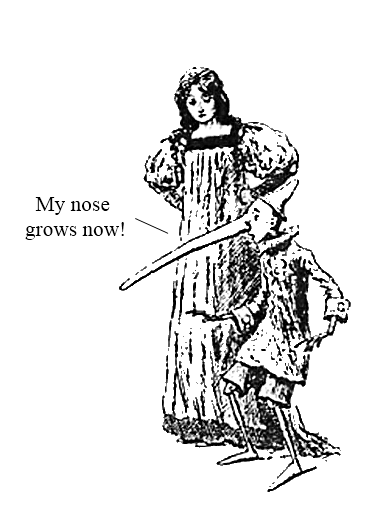
\includegraphics[height=30ex]{res/Pinocchio_paradox.png}
  \caption{Pinocchio says a lie and stretches his nose}
  \label{fig:Pinocchio}
\end{figure}

\begin{thm}
    The halting problem is undecidable.
\end{thm}
\begin{proof}
    Assume there exists a Turing machine $\mathbb B$ that decides the
    halting problem i.e.~for all Turing machines $\mathbb A$ and all
    strings $x$

    \[ \mathbb B(\enc{\mathbb A}, x) =
    \begin{cases}
      \one  & \text{if } \mathbb A \text{ halts on } x\\
      \zer  & \text{if } \mathbb A \text{ does not halt on } x
    \end{cases}\]

    Now using $\mathbb B$ construct a Turing machine $\mathbb B'$ that
    simulates $\mathbb B(\enc{\mathbb A}, \enc{\mathbb A})$ on its input
    $\enc{\mathbb A}$ and enters an infinite loop if
    $\mathbb B(\enc{\mathbb A}, \enc{\mathbb A}) = \zer$. Expressed more
    formally this means

    \[
      \mathbb B' \text{ halts on } \enc{\mathbb A} ⇔
      \mathbb A \text{ does not halts on } \enc{\mathbb A}.
    \]

    Setting $\mathbb A = \mathbb B'$ yields the desired contradiction.
\end{proof}

For a more detailed proof of this fact and lot more information on computability
see \cite{Cooper2004}. As the halting problem is undecidable the halting set
defined by
\[
 \mathcal{K} = \set{⟨\enc{\mathbb A}, x⟩ \mid \mathbb A \text{ halts on } x}
\]
is undecidable. However using the universal Turing machine it is clearly
semi-decidable.
